\section{Communication Framework}
\label{sect:comms}

The \ngrm\ architecture is hierarchical and recursive
(\ref{ReqsHiLevFun}, req. 4.1).
A root instance of \ngrm\ contains all the
idle resources.  A job spawned by the root instance contains
its own \ngrm\ instance, which may in turn spawn jobs, ad infinitum.
When a job terminates, the job's instance terminates and resources
return to the parent instance.

The communication framework supports this architecture by
establishing a {\em comms session}\footnote{{\em Comms} is a shorthand
for \ngrm\ Communications Framework and is not related to MPI communicators.}
to contain each \ngrm\ instance
and provide a foundation for the distributed components of \ngrm\ to
be built upon.
The framework enables secure, scalable communication
within a comms session, limits communication between sessions,
and allows new comms sessions to be created, resized, destroyed,
and monitored by existing ones in a parent-child relationship.
\ifcomments
\marginpar{\tiny {\bf ned-review:}
A worked example would be useful here.
{\bf jg:} for now, section~\ref{sect:monitor} might be helpful.}
\fi

A comms session is only ``aware'' of its parent and immediate offspring.
Any communication between siblings would have to be orchestrated by
the parent.  This sandboxing arrangement should encourage the higher level
components of \ngrm\ 
to be built so they can operate at any level of recursion, thus improving
their testability and making development of replacement components easier.

It should be noted that although \ngrm\ obtains scalability from the job
hierarchy, the {\em idle} root comms session must contain all the systems and
resources managed by \ngrm\ and therefore must handle the full 100,000 node
scalability target (\ref{ReqsHiLev}).

The communication framework consists of four main layers:
IP protocols and services, comms toolkit, comms message broker, and
reduction network, shown
in Figure~\ref{FigCommsLayers}.  Layering is not rigid;
that is, higher level \ngrm\ components can use any of the
layers directly as appropriate\footnote{At this stage in the design of \ngrm,
we do not wish to overly constrain the solution space for the other
components that will use the comms framework.  For the same reason,
distributed object oriented frameworks, such as those derived from
CORBA, were rejected as too confining.  This stance can be re-evaluated
as the other components are designed.}.

\begin{figure}
\begin{minipage}[b]{0.45\linewidth}
\centering
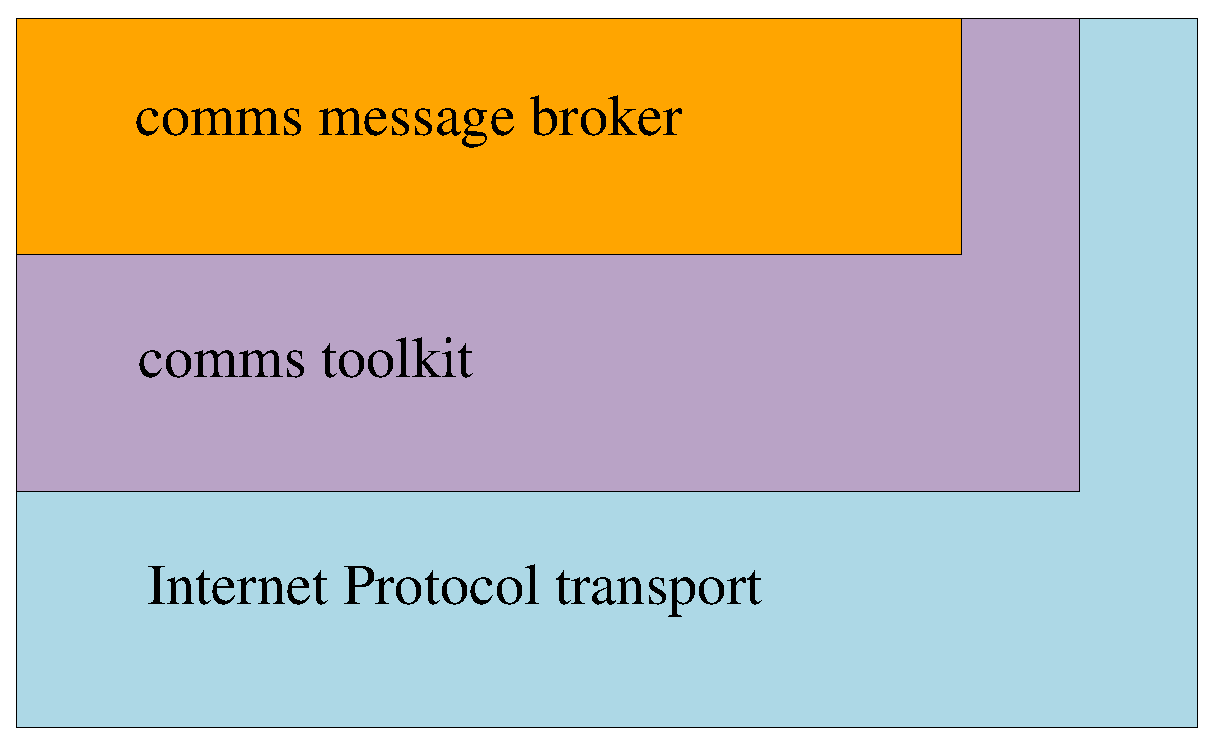
\includegraphics[scale=0.30]{comms}
\caption{Communication Framework Layers}
\label{FigCommsLayers}
\end{minipage}
\hspace{0.5cm}
\begin{minipage}[b]{0.45\linewidth}
\centering
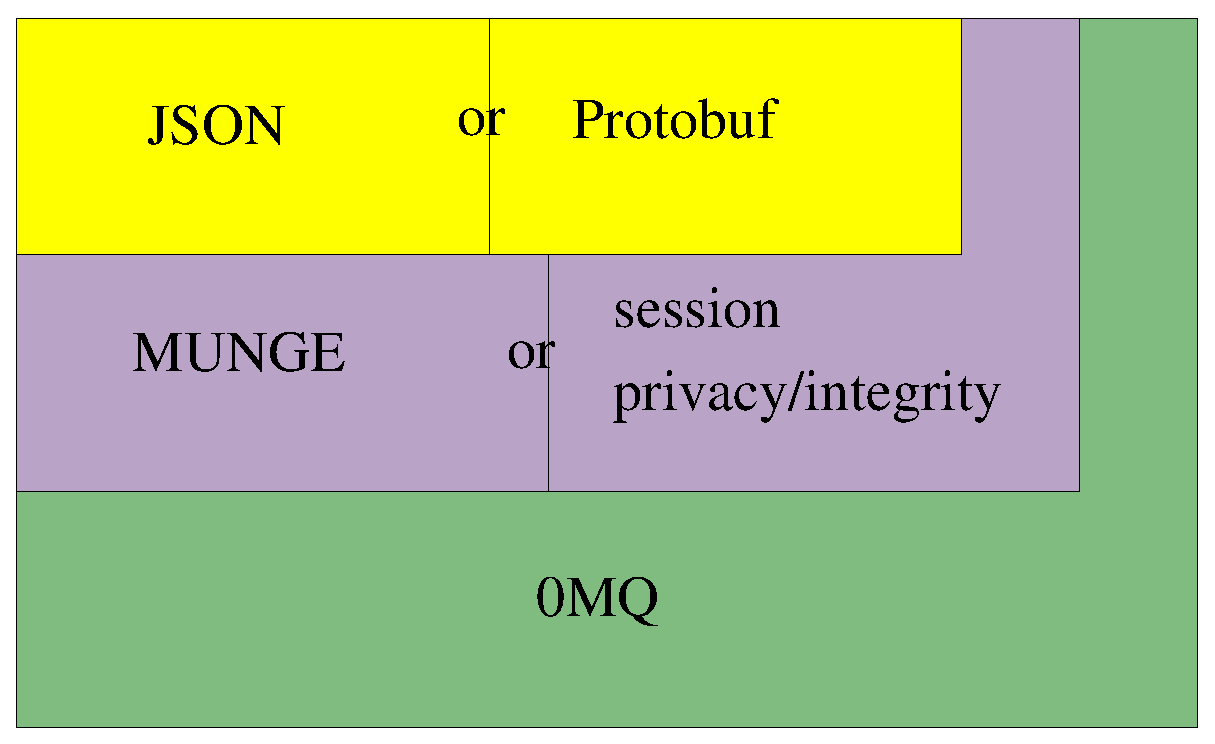
\includegraphics[scale=0.30]{commstk}
\caption{Comms Toolkit Layers}
\label{FigCommsTK}
\end{minipage}
\end{figure}

\subsection{Internet Protocols and Services}
\label{sect:commsIP}

The \ngrm\ comms framework is layered upon Internet Protocol (IP)\footnote{
The low-latency and low-overhead bulk transfer properties of RDMA
communications such as provided by Common Communication
Interface (CCI) were considered and rejected as unnecessary for \ngrm.}
and presumes complete IP level unicast and multicast connectivity across
participating systems, so that any
collection of nodes can be wired up in a comms session without
the need to re-implement the equivalent of IP routing within
the framework.\footnote{Building a reliable 100K node IP internetwork
is a solved problem.  Building a hardened overlay network with similar
properties is difficult and would limit our ability to leverage
other software built on IP.}
The addressing, routing, and subnetting of this IP network is beyond of
scope of \ngrm, except that its design should introduce no single
points of failure (\ref{ReqsHiLevFun}, req. 1.2)
and should avoid performance bottlenecks which
would unnecessarily constrain the resource manager's node selection options.

The comms framework should support communication over multiple
(fully-routed) network planes, for example using either a management
ethernet or IP-over-IB or both according to the performance/reliability
requirements of the particular application.

Dynamic unicast IP address allocation must be available to support
dynamically created virtual nodes (Linux containers launched with
virtual network interfaces).  In fact, it is worth noting here that
we expect to make heavy use of virtual nodes in \ngrm\ for our internal
services that should not be co-located with computation.
Similarly,
dynamic multicast address allocation must be available to support
private multicast groups within dynamically created comms sessions.
These requirements can be addressed by existing technology such as
DHCP~\cite{rfc2131} and MADCAP~\cite{rfc2730}.

\ifcomments
\marginpar{\tiny {\bf ned-review:}
Would we point resolvers ouside \ngrm\ at the NGRM internal DNS?
{\bf jg:} I envision NGRM operating in a private network.
In that case, resolving private addresses from outside doesn't seem useful.
However, we may want to consider whether we need some way to map external
addresses with names to internal ones.}
\fi
A private DNS~\cite{rfc1034} is used by the comms framework to
map a hierarchical namespace to the comms session hierarchy.
The root comms session has the root domain name, e.g. ``{\tt \ngrm.}'',
and the root server contains address records for all hosts in the domain, e.g.
``{\tt n1.\ngrm}'', ``{\tt n2.\ngrm}'',..., ``{\tt n99999.\ngrm}''.
Comms sessions spawned by the root session get their own sub-domain, e.g.
``{\tt s1.\ngrm}'', ``{\tt s2.\ngrm}'', ``{\tt s3.\ngrm}'',
and contain address records for the nodes assigned to them, e.g.
``{\tt n1.s1.\ngrm}'', ``{\tt n2.s1.\ngrm}'', ``{\tt n3.s1.\ngrm}''.
Sub-domains are created for each level of comms session recursion.
Each session runs a set of DNS servers for its domain.
When a node joins a new session, its DNS resolver is reconfigured to use
the session DNS servers and to search the session's DNS domain first,
thus each level of session overlays a new set of names over
the root session's that provides job-centric naming uniformity.
DNS SRV records~\cite{rfc2782} provide a rudimentary service location
brokerage within the session.
Well understood techniques for DNS fault tolerance,
caching, and dynamic reconfiguration are leveraged to scale performance
in large sessions such as the root session.

A comms session could optionally be spawned inside a virtual private
network (\ref{ReqsUseCases}, UC21) such that IP communication
is limited to within the comms session.  IPsec~\cite{rfc2401} with
a pre-shared session key could be used to provide session integrity and
privacy at the IP layer if desired.

\subsection{Comms Toolkit}

The framework provides a toolkit for sending and receiving
protocol messages privately and securely within a session,
with the goals of providing a robust foundation for \ngrm\ components
and promoting rapid development, code reuse, and interoperability.
The toolkit includes messaging libraries,
protocol encoding/decoding libraries, and security options.
Toolkit pieces can be mixed and matched according to application
requirements.  We may cull the comms toolkit as we learn more
about the pieces while prototyping other \ngrm\ components.

\begin{figure}
\centering
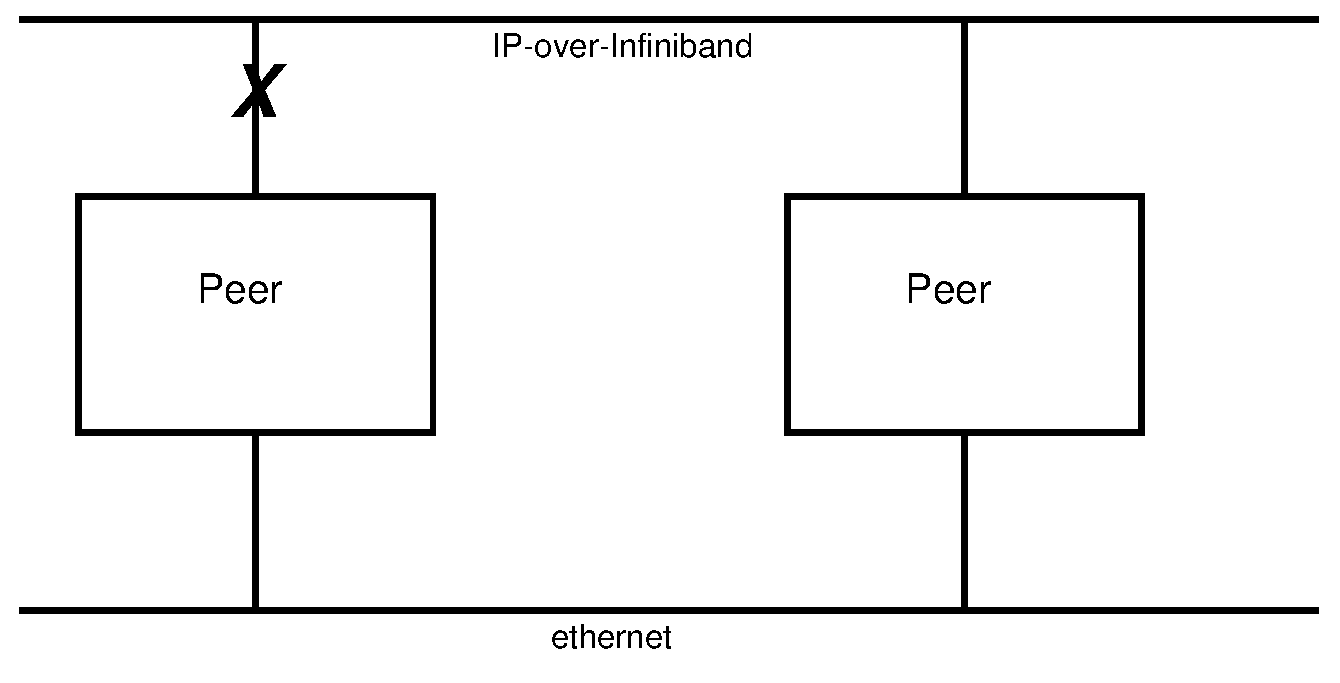
\includegraphics[scale=0.3]{comms_sctp}
\caption{SCTP supports transparent multi-homing of one socket over multiple
network planes, for example using both Infiniband and Ethernet in a cluster.
If one network drops a packet, it is retransmitted on the other, which with
proper tuning, improves both availability and responsiveness compared with
TCP single-homed sockets.}
\label{FigCommsSCTP}
\end{figure}

\begin{figure}
\begin{minipage}[b]{0.15\linewidth}
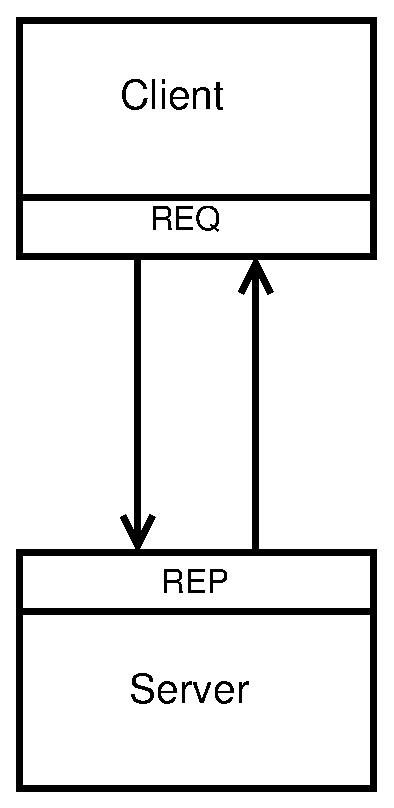
\includegraphics[scale=0.3]{comms_zmq_reqrep}
\end{minipage}
\hspace{0.5cm}
\begin{minipage}[b]{0.4\linewidth}
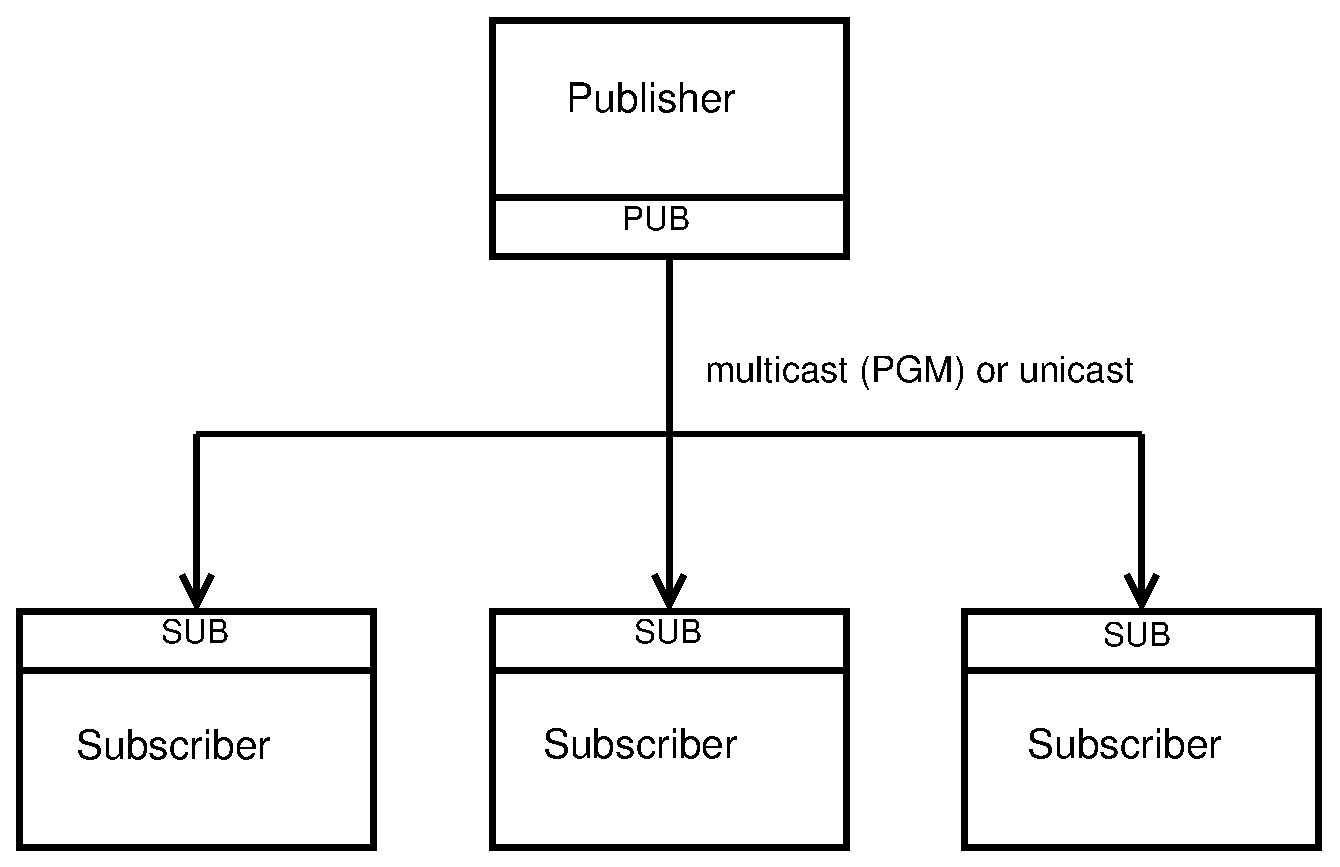
\includegraphics[scale=0.3]{comms_zmq_pubsub}
\end{minipage}
\hspace{0.5cm}
\begin{minipage}[b]{0.4\linewidth}
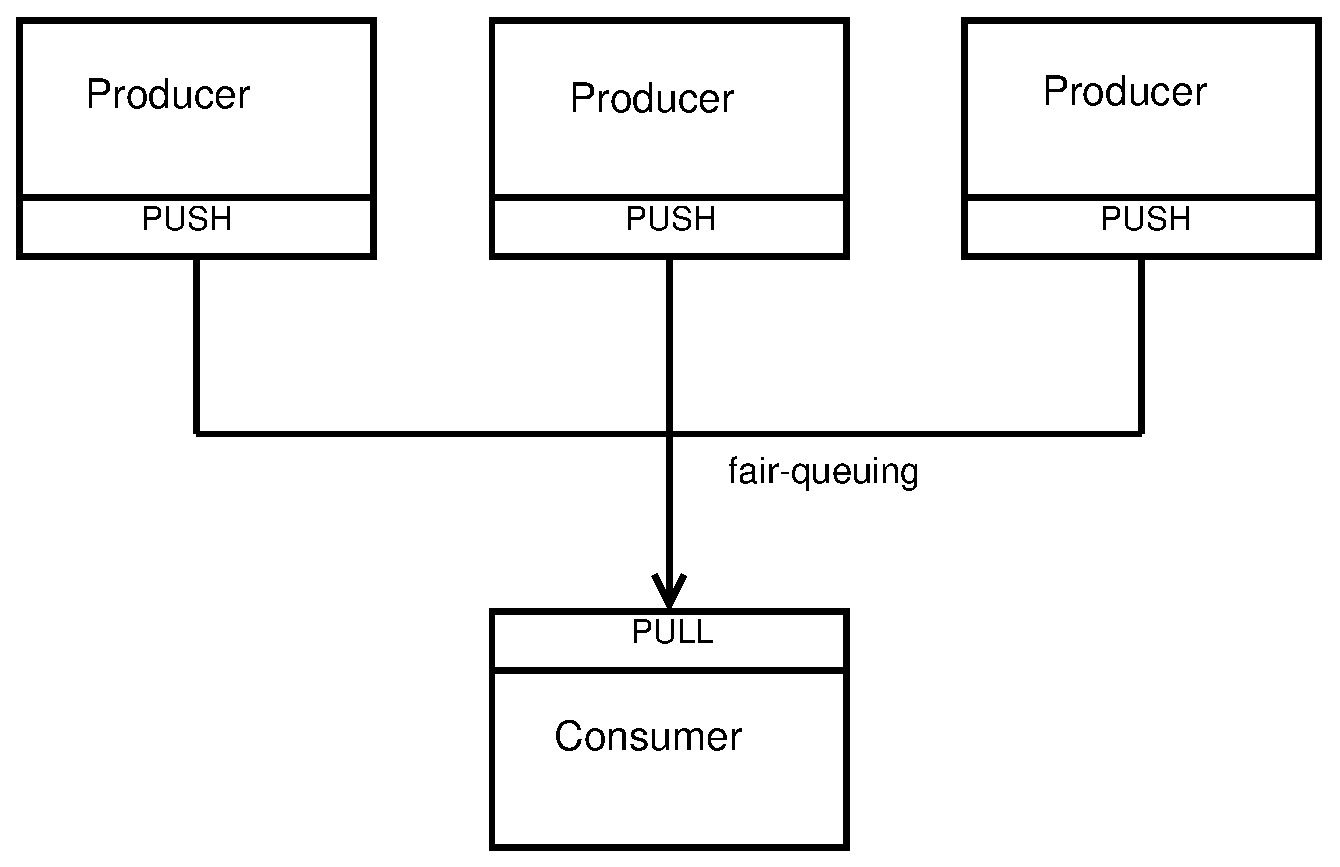
\includegraphics[scale=0.3]{comms_zmq_pushpull}
\end{minipage}
\caption{\zMQ\ provides a sockets-like API that supports several
messaging patterns including REQ-REP, PUB-SUB, and PUSH-PULL.
These basic patterns are complemented by other patterns used when
building distributed message brokers.  For example, XPUB-XSUB handles
subscription forwarding to optimize multi-level broker based
publish-subscribe networks.}
\label{FigCommsZmq}
\end{figure}

Two messaging approaches of interest are \zMQ~\cite{ZMQGuide} and
SCTP~\cite{SCTP}.
\zMQ\ provides the ability to manipulate opaque, multipart messages,
and carry them across various transports, including TCP and
PGM~\cite{rfc3208} (reliable multicast), using a socket-like API.
\zMQ\ sockets can exchange messages using patterns including
REQ-REP (RPC), PUB-SUB, and PUSH-PULL (message stream).
\zMQ\ can be used to build applications or custom message brokers.
Complex message routing topologies such as tree-based overlay networks
(Figure~\ref{FigZmqTBON}) can be built from simple components.
\zMQ\ has a large number of language bindings.

SCTP is an IETF-standardized, message-oriented transport developed
in the telephony world with an implementation in the Linux kernel.
It offers multi-streaming, the bundling of {\em streams} in one
{\em association} (connection).  Individual streams can be configured for
different ordering and reliability semantics.  SCTP supports
multi-homing for reliability and congestion avoidance, as shown in
Figure~\ref{FigCommsSCTP}, and
can transparently generate and check an HMAC for messages using a
pre-shared key to implement message integrity.  Unlike \zMQ, SCTP is
connection-based and does not implement a standardized reliable multicast
mode.

Two widely used methods of encoding data in messages are
JSON~\cite{rfc4627} 
and Protocol Buffers~\cite{Protobuf}.
JSON is a self-describing format
that supports protocol evolution without recompiling endpoints.  It has
many language bindings but it is also space-inefficient and slow.
Protocol Buffers is a compiled format that supports
only limited protocol evolution without recompilation.  It has relatively
fewer language bindings than JSON but is space-efficient and fast.
Depending on the application either may be appropriate.

Message integrity and privacy can be obtained using either a session
security context or via MUNGE~\cite{MUNGE}.
Each comms session is allocated a {\em session key} by its parent
which is used for establishing a shared security context
for messages exchanged within the comms session.
The shared security context allows communicating entities to have integrity
and privacy (from children, siblings, and their children)
without the overhead
of a key exchange for each pair of communicating endpoints.
This is especially useful for non point-to-point comms patterns such as PUB-SUB.
The parent retains state about its offspring including their session keys.
Children forget their parent's key;  thus as comms sessions recurse,
parents get privacy from children but not the reverse.
An application acting as a gateway between parent and child would use
the child's session key as it is known by both parent and child.

If the sender of a message needs to be authenticated, or if messages must
be kept private from other users within the session or its anscestors,
messages can be enclosed as payload in a MUNGE~\cite{MUNGE}
credential.
In order for this to work, \ngrm's comms framework must operate within a
single MUNGE security realm,
which implies a single administrative domain with consistent
user and group identities.
\newpage
\subsection{Comms Message Broker}
\label{sect:cmb}

Within a comms session, a distributed comms message broker (CMB)
is established to provide basic session services.
The CMB is responsible for launching new sessions,
managing session membership,
detecting and adapting to session node failures,
providing a basic event messaging system,
and starting other \ngrm\ components.

\begin{figure}
\begin{minipage}[b]{0.2\linewidth}
\fbox{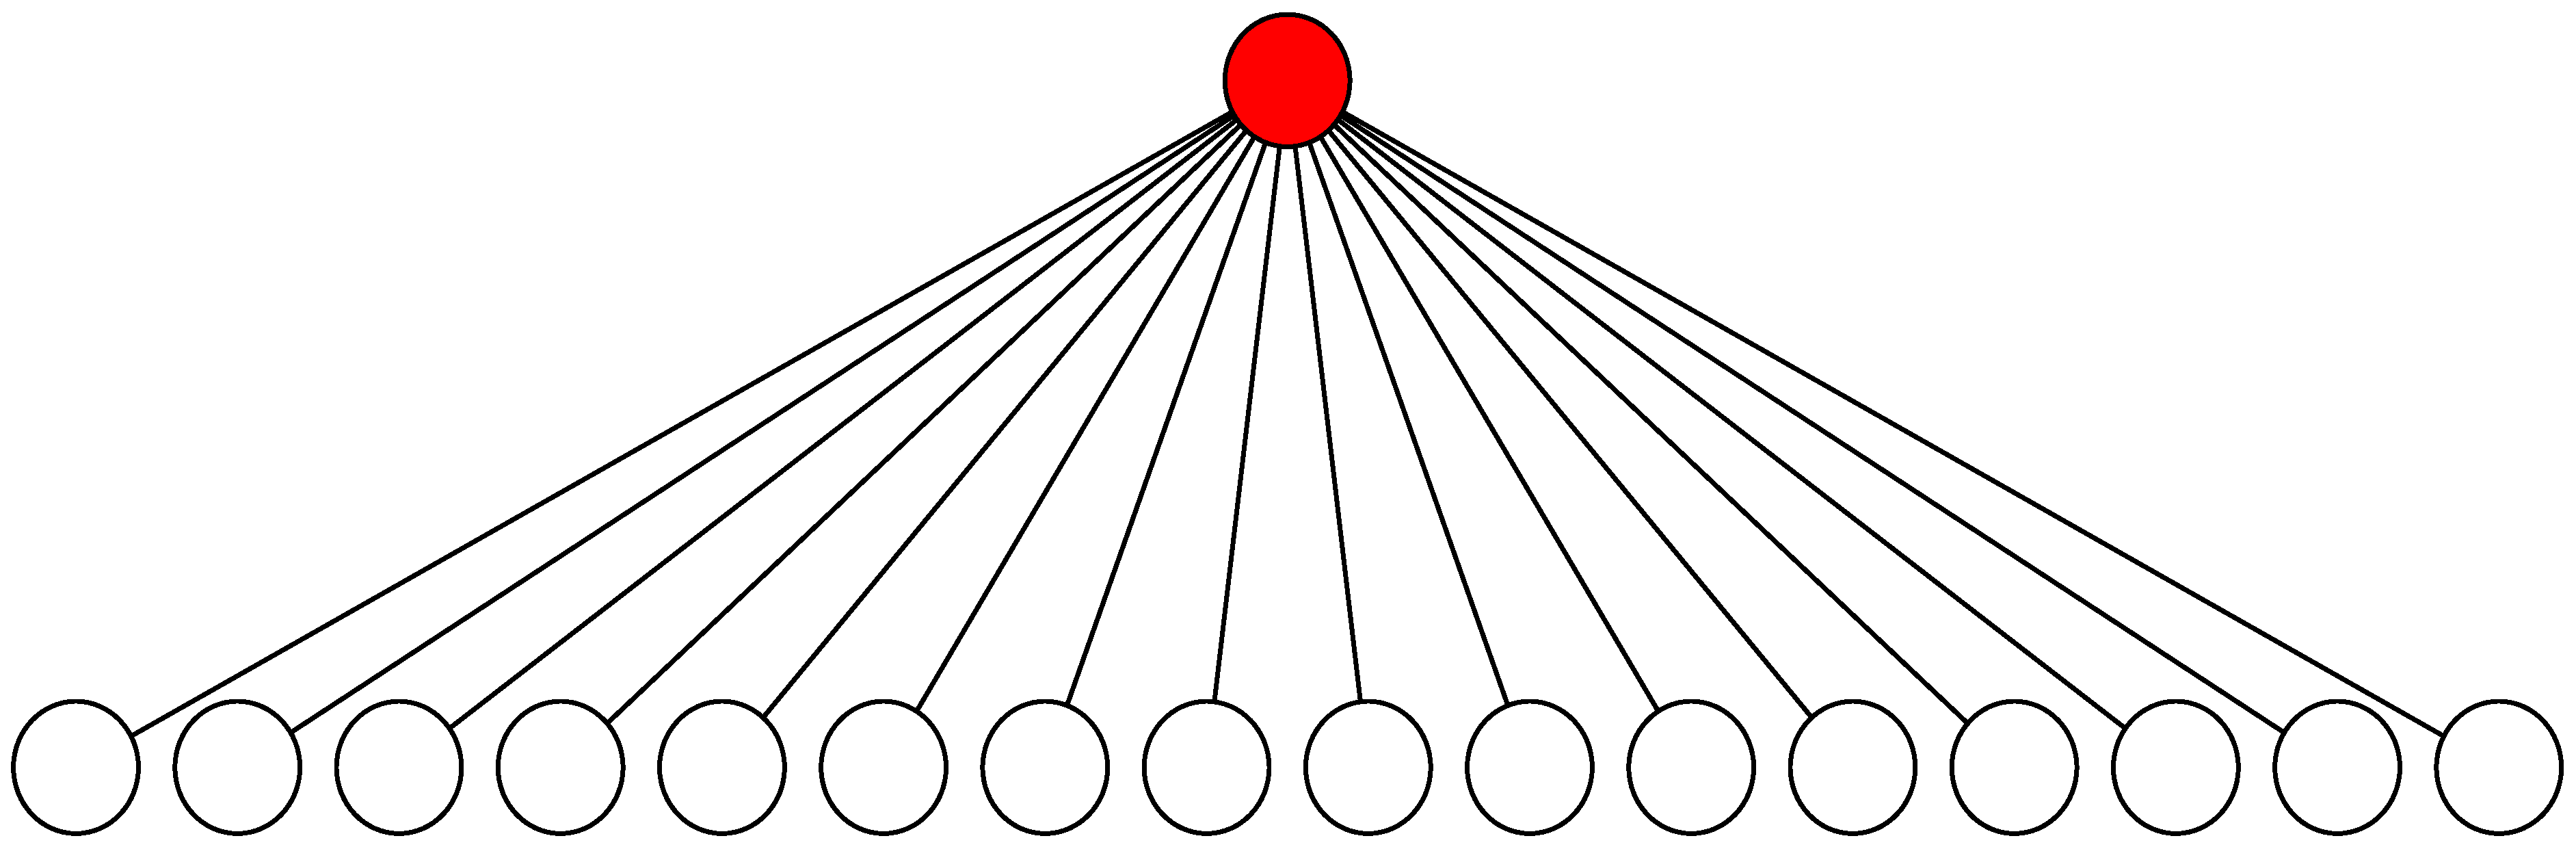
\includegraphics[scale=0.05]{comms_ex1a}}
\end{minipage}
\hspace{0.5cm}
\begin{minipage}[b]{0.2\linewidth}
\fbox{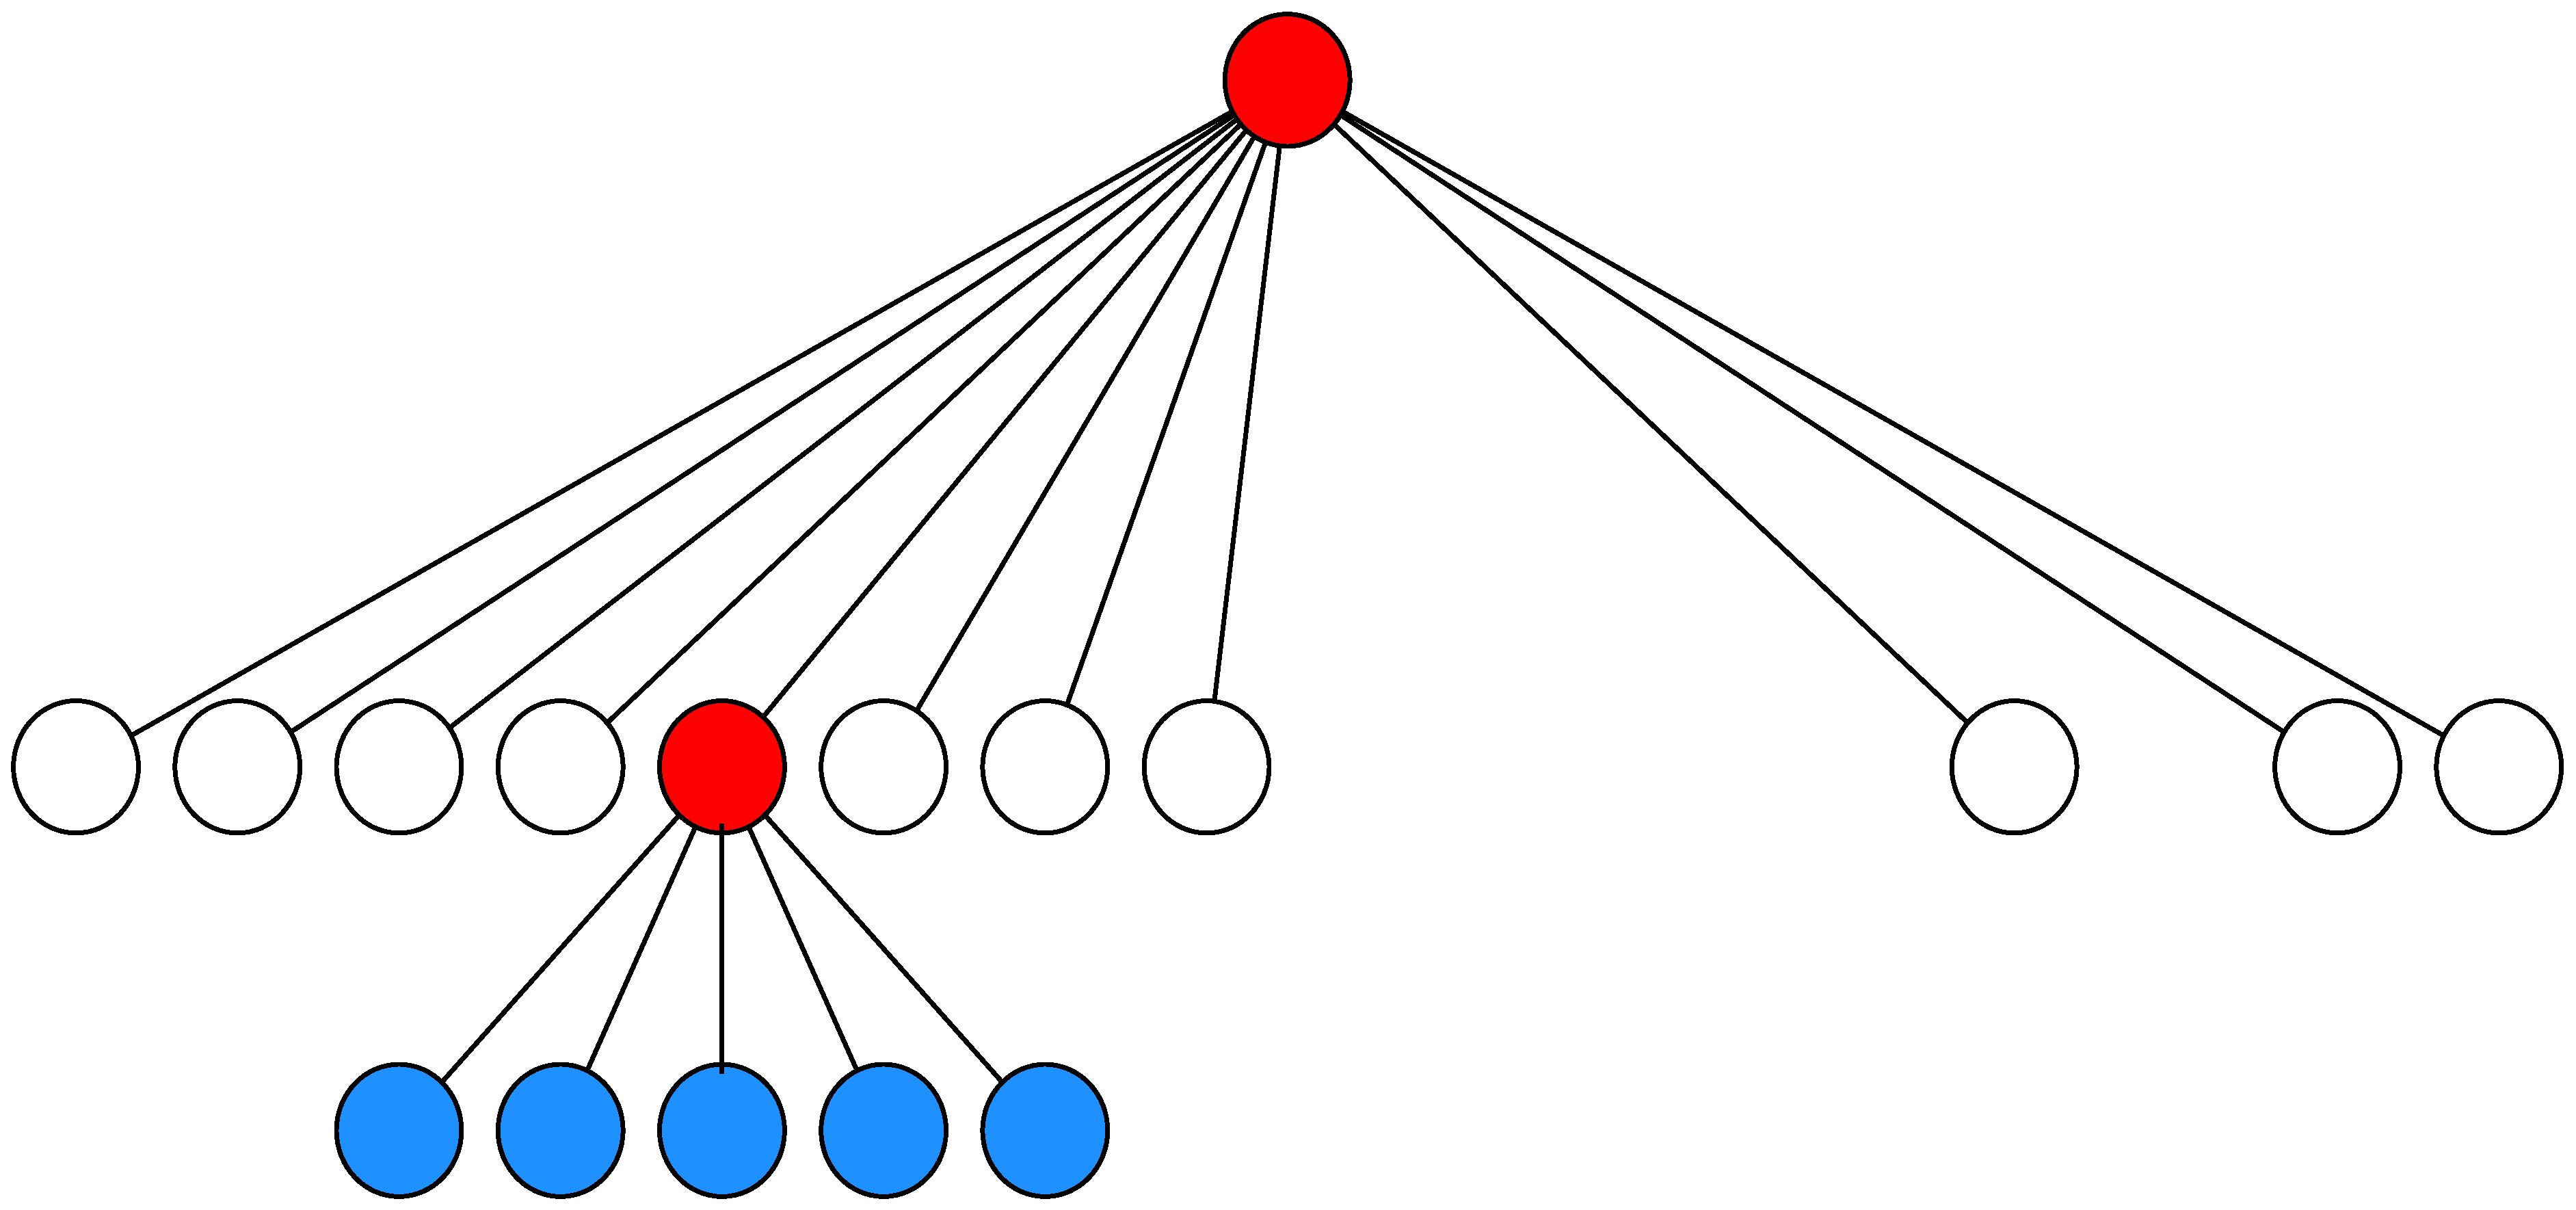
\includegraphics[scale=0.05]{comms_ex1b}}
\end{minipage}
\hspace{0.5cm}
\begin{minipage}[b]{0.2\linewidth}
\fbox{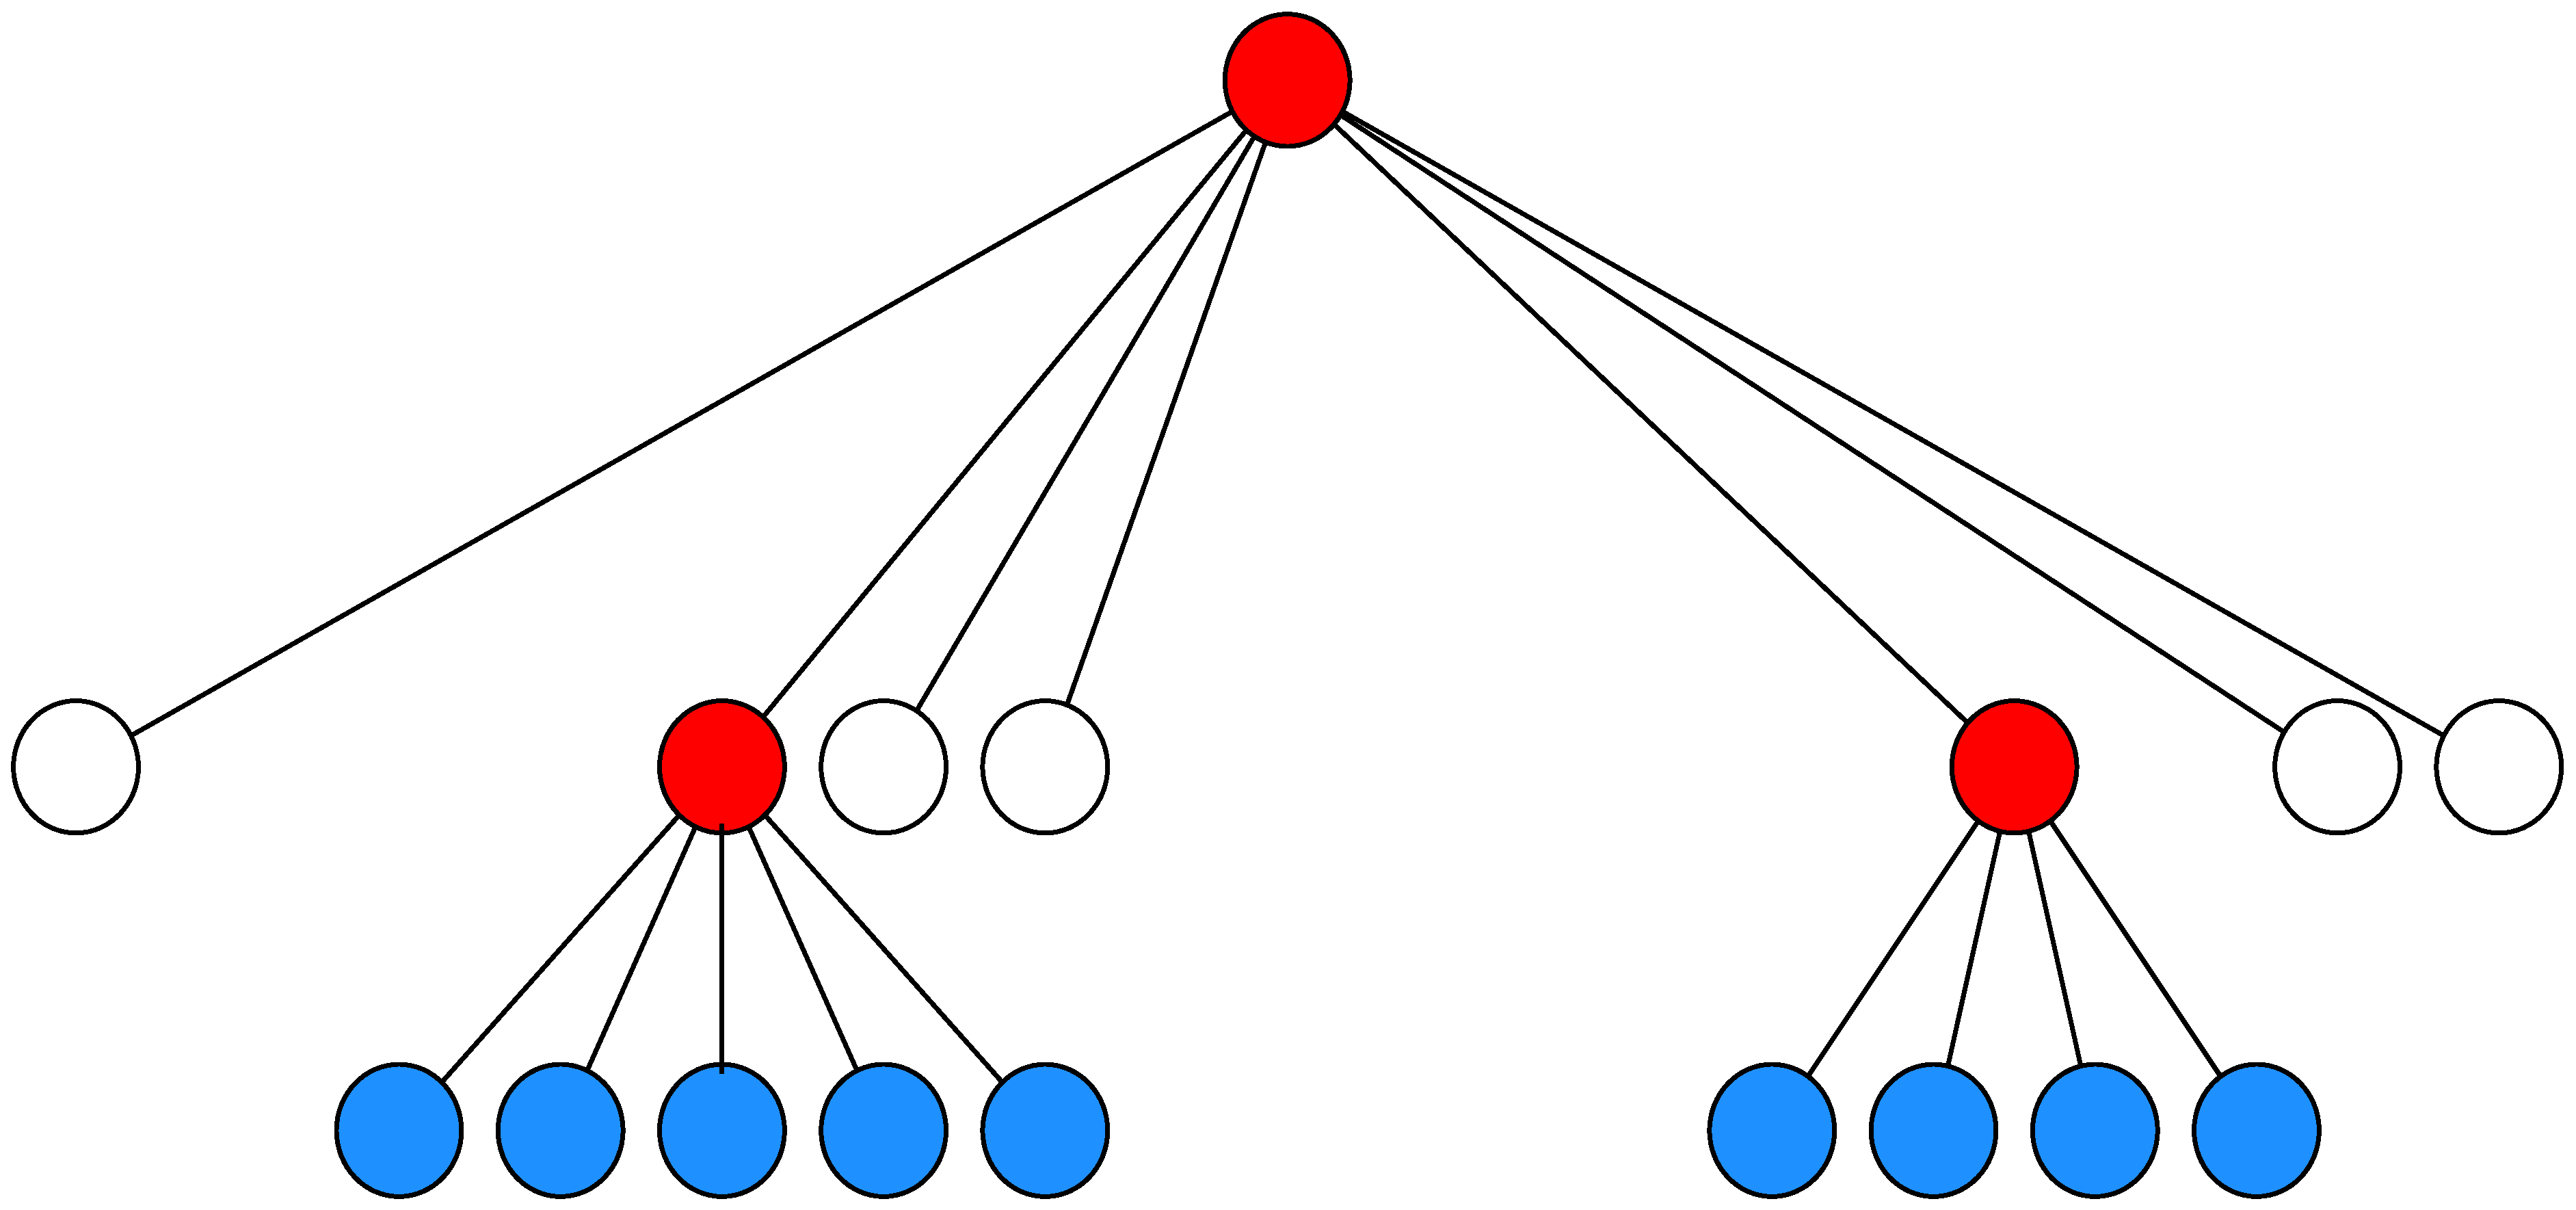
\includegraphics[scale=0.05]{comms_ex1c}}
\end{minipage}
\hspace{0.5cm}
\begin{minipage}[b]{0.2\linewidth}
\fbox{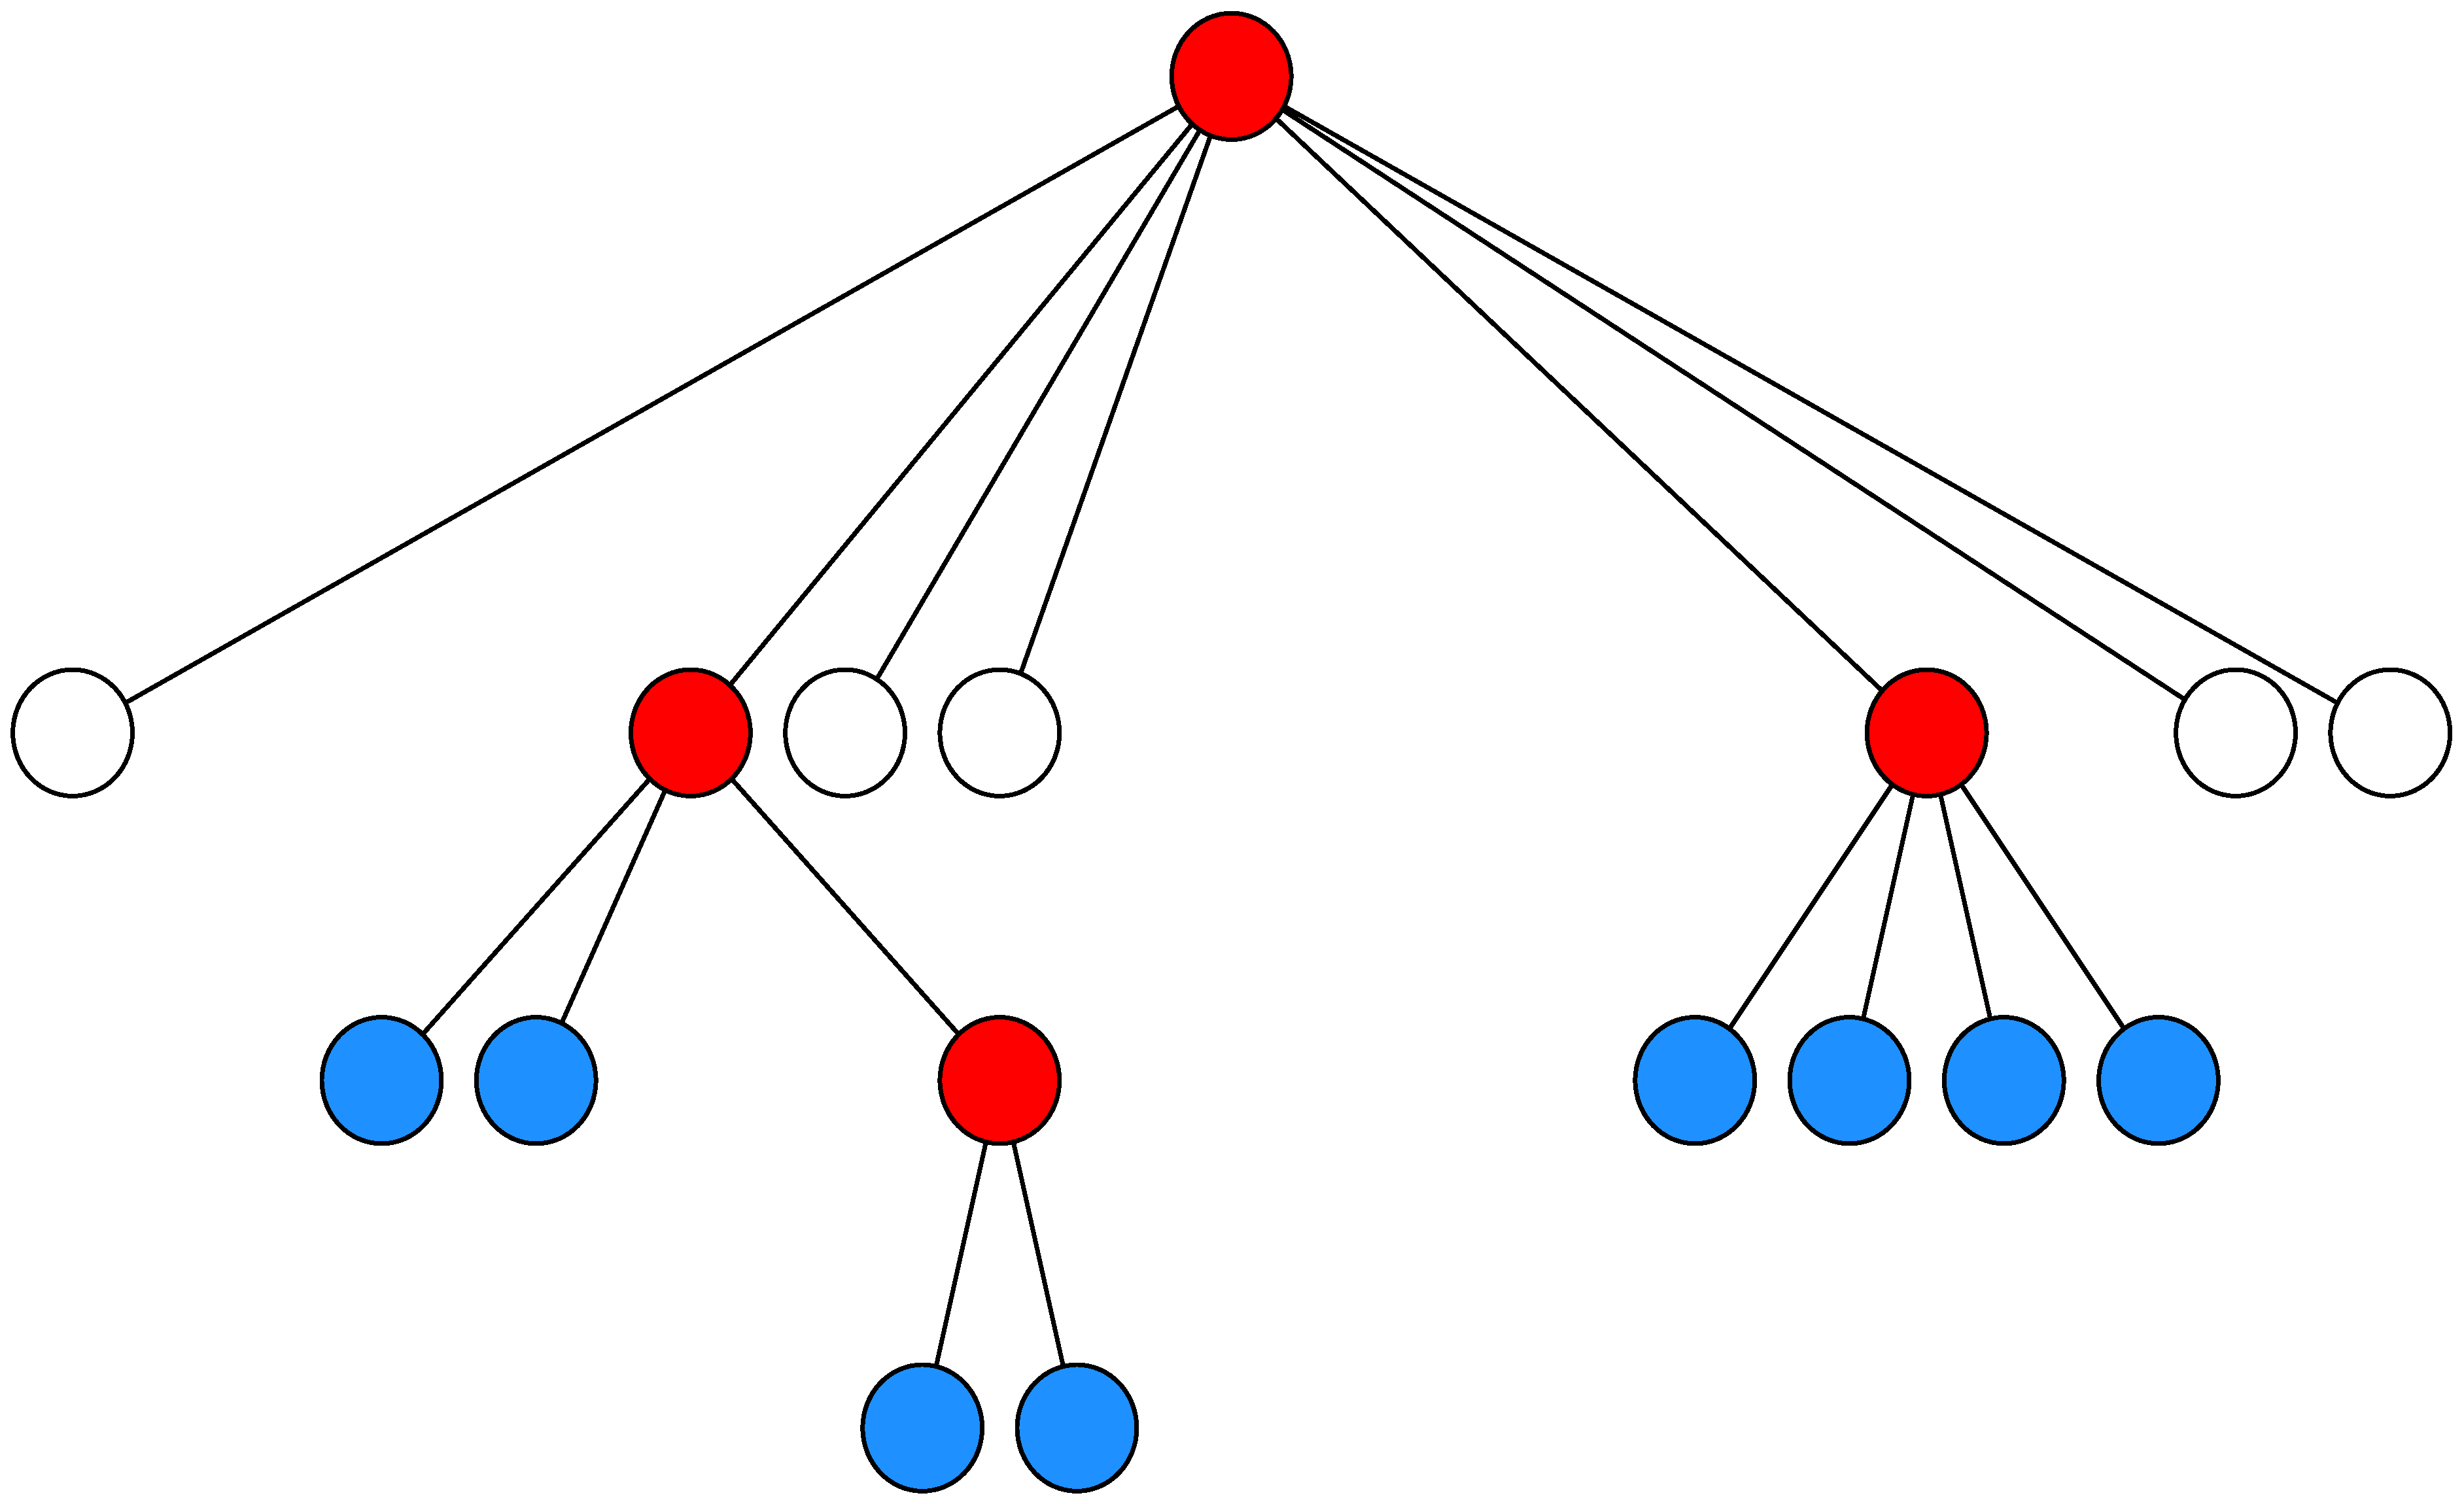
\includegraphics[scale=0.05]{comms_ex1d}}
\end{minipage}
\caption{CMB Architecture:  comms sessions are formed hierarchically.
Session control nodes (red) are the interface between a session and its parent.
An idle root session is shown on the left; one and two sessions running 
work (blue) under the root are shown in the middle, and one of those has
spawned a child on the right.  Note that although control nodes are depicted
as being allocated from real nodes, depending on the session size, they may
be created on demand as virtual nodes.}
\label{FigCommsEx1}
\end{figure}

\paragraph{Architecture}
The CMB is a distributed service with nodes interconnected in a tree-based
topology.
A distinguished {\em control node} serves as the heart of the CMB
and the root of the tree.
The control node is distinguished because it alone communicates with
the parent session, and it holds the master copy of the session state.
% XXX: see sec 6.4 - children may need to subscribe to parent changes
% such as draining of a resource
%Interfaces exposed by the control node to the parent are always passive;
%that is, the parent initiates connections and makes requests or subscribes
%to events, and the child control node responds or publishes events.
The hierarchical relationship between comms sessions with the control
node acting as gateway is depicted in Figure~\ref{FigCommsEx1}.
The details of any internal tree-based interconnections
are not depicted in the figure, and are a future design activity.

\paragraph{Session State}
The CMB implements a simple key-value store to manage the
internal state enumerated in Table~\ref{TabCMBState}.
The session state for the largest session is small enough to easily
fit in memory.
The master state for a session lives on the session control node.
Slave caches on other nodes in the session are loosely consistent with
the master copy; that is, reads may utilize a local or peer cache,
which may be slightly out of date relative to the master copy,
while writes are through to the control node.
Each write on the control node updates the key's generation number,
its value, and triggers a state update event which
can be used to update caches and synchronize other software using the
state.  If the control node crashes, state can be recovered from
one of the slave caches.\footnote{The fault tolerance strategy here is to
be designed.  One approach is that the parent can determine if a control
has stop functioning (see {\em Liveness Monitoring} below) and intervene
to establish a new one with restored state from slave caches.}

\begin{table}
  \centering
  \begin{tabular}{| l | p{0.6\textwidth} |}\hline
  \textbf{Name} & \textbf{Description} \\
  \hline
  cmb.cred = $key$ &
        My session key.\\
  cmb.fqdn = $name$ &
        Fully qualified domain name for the session.\\
  cmb.nodeset = $nodelist$ &
        List of my nodes.\\
  cmb.addrs.$node$ = $addrs$ &
        List of addresses for $node$, for forming DNS address records.\\
  cmb.topology.up.$node$ = $nodelist$ & 
        Upward peers for $node$ in CMB topology.\\
  cmb.topology.dn.$node$ = $nodelist$ &
        Downward peers for $node$ in CMB topology.\\
  cmb.alive.$node$ = $yes|no$ &
        Liveness for $node$.\\
  cmb.alloc.$node$ = $yes|no$ &
        Allocation status for $node$.\\
  cmb.attrs.$node$ = $attrlist$ &
	Role attributes assigned to $node$, e.g. ``dns'' and ``control''.\\
  cmb.subscribe.$key$ = $nodelist$ &
        List of nodes subscribed to $key$.\\
  cmb.exec = $cmdline$ &
        Executable to bootstrap on each node.\\
  \hline
  cmb.child.sessions = $sessions$ &
        List of active child sessions.\\
  cmb.child.$session$.cred = $key$ &
        Child sesion key.\\
  cmb.child.$session$.control = $nodelist$ &
        Control node(s) for $session$.\\
  cmb.child.$session$.dns = $nodelist$ &
        DNS server nodes for $session$, for forming DNS NS records.\\
  \hline
  \end{tabular}
  \caption{A small amount of data comprises the comms session state,
	   which is stored in a simple key-value store replicated across
	   the session.}
  \label{TabCMBState}
\end{table}

\paragraph{Event Messaging}
\ifcomments
\marginpar{\tiny {\bf FIXME:}
The per-job scheduling trigger probably has insufficient emphasis here.
It is an important benefit that reduces our noise footprint and
could be generally useful to other system/tools software written
to run within a job.}
\fi
The CMB implements a session-wide event messaging service.
Clients of the CMB on any node can publish a $(tag, message)$ event tuple.
Other clients can subscribe to events by tag.  The CMB ensures that
event messages are routed internally from publishers to subscribers.
The event service is reliable, and for events originating on the same node,
sequenced for in-order delivery.
Events are not queued for late subscribers.
There is a special {\tt event.sched.trigger} event sent out periodically
to synchronize the CMB's internal functions (and those of any other
subscribers to the event) across the session with the goal of minimizing
disruption to bulk-synchronous workloads running within the session.

\paragraph{Session Membership}
The CMB maintains the current {\em nodeset} as part of the session state.
The CMB arranges for the nodeset to be mirrored in private DNS servers
serving up the session's subdomain.
The nodeset may grow or shrink in response to higher level software
allocating/freeing nodes from the parent, or creating/destroying 
virtual nodes within the session.
Nodeset updates will be accompanied by internal topology updates, provided by
the software making the nodeset change or by the CMB itself depending
on the situation.
State update events will be published for the nodeset and topology changes.
While nodes are allocated to a session, they remain in the parent nodeset,
tagged as {\em allocated}.  They forget the parent's session state and key.
When nodes are freed back to the parent, the parent CMB, having subscribed
to the child's nodeset update events, contacts the freed node (using the
child session key) and brings it back online in the parent sesssion.  

\paragraph{Liveness Monitoring}
The CMB maintains the {\em liveness} of its nodes as part
of the session state.
Liveness is assessed by forcing member nodes to communicate with the CMB
at minimum intervals, synchronized by the aforementioned trigger event.
If the CMB has not heard from a node for some number
of trigger periods, it is marked down.
If it finally is heard from, it is marked {\em up}.
In some cases the CMB control node may adjust its internal topology
to account for such changes.
As described above, session state changes trigger state change events.
Higher level software wishing to react to node liveness changes can
subscribe to state change events.
The parent continues to track liveness of nodes allocated to a child by
subscribing to liveness updates via the child's control node.  A trivial
utility that asks the CMB for a list of down nodes in the current session
and all of its progeny can be written that works equally well at any level of recursion,
even at the level of the root session.

\paragraph{Node Bootstrap}
A cold started node (or restarted CMB daemon) joins the root session,
obtaining the root session key and the identity of a peer to copy the
session state from out of band in a secure manner.
If the CMB is cold starting after crashing while assigned to
a session other than the root, the CMB of the root and subsequent owning
sessions re-add the node from child to child until there are no children
left or it is evicted according to the policy of an owning session
at any level of hierarchy.

\paragraph{Executable Bootstrap}
In order to bootstrap other \ngrm\ components, the CMB daemon, upon
joining a new session, launches a single process on each node,
determined by the {\tt cmb.exec} state variable.
This process is terminated when the node alters its session membership
to join a child session or return to a parent session.
If the process terminates early, an event is generated.

%\begin{figure}
%\centering
%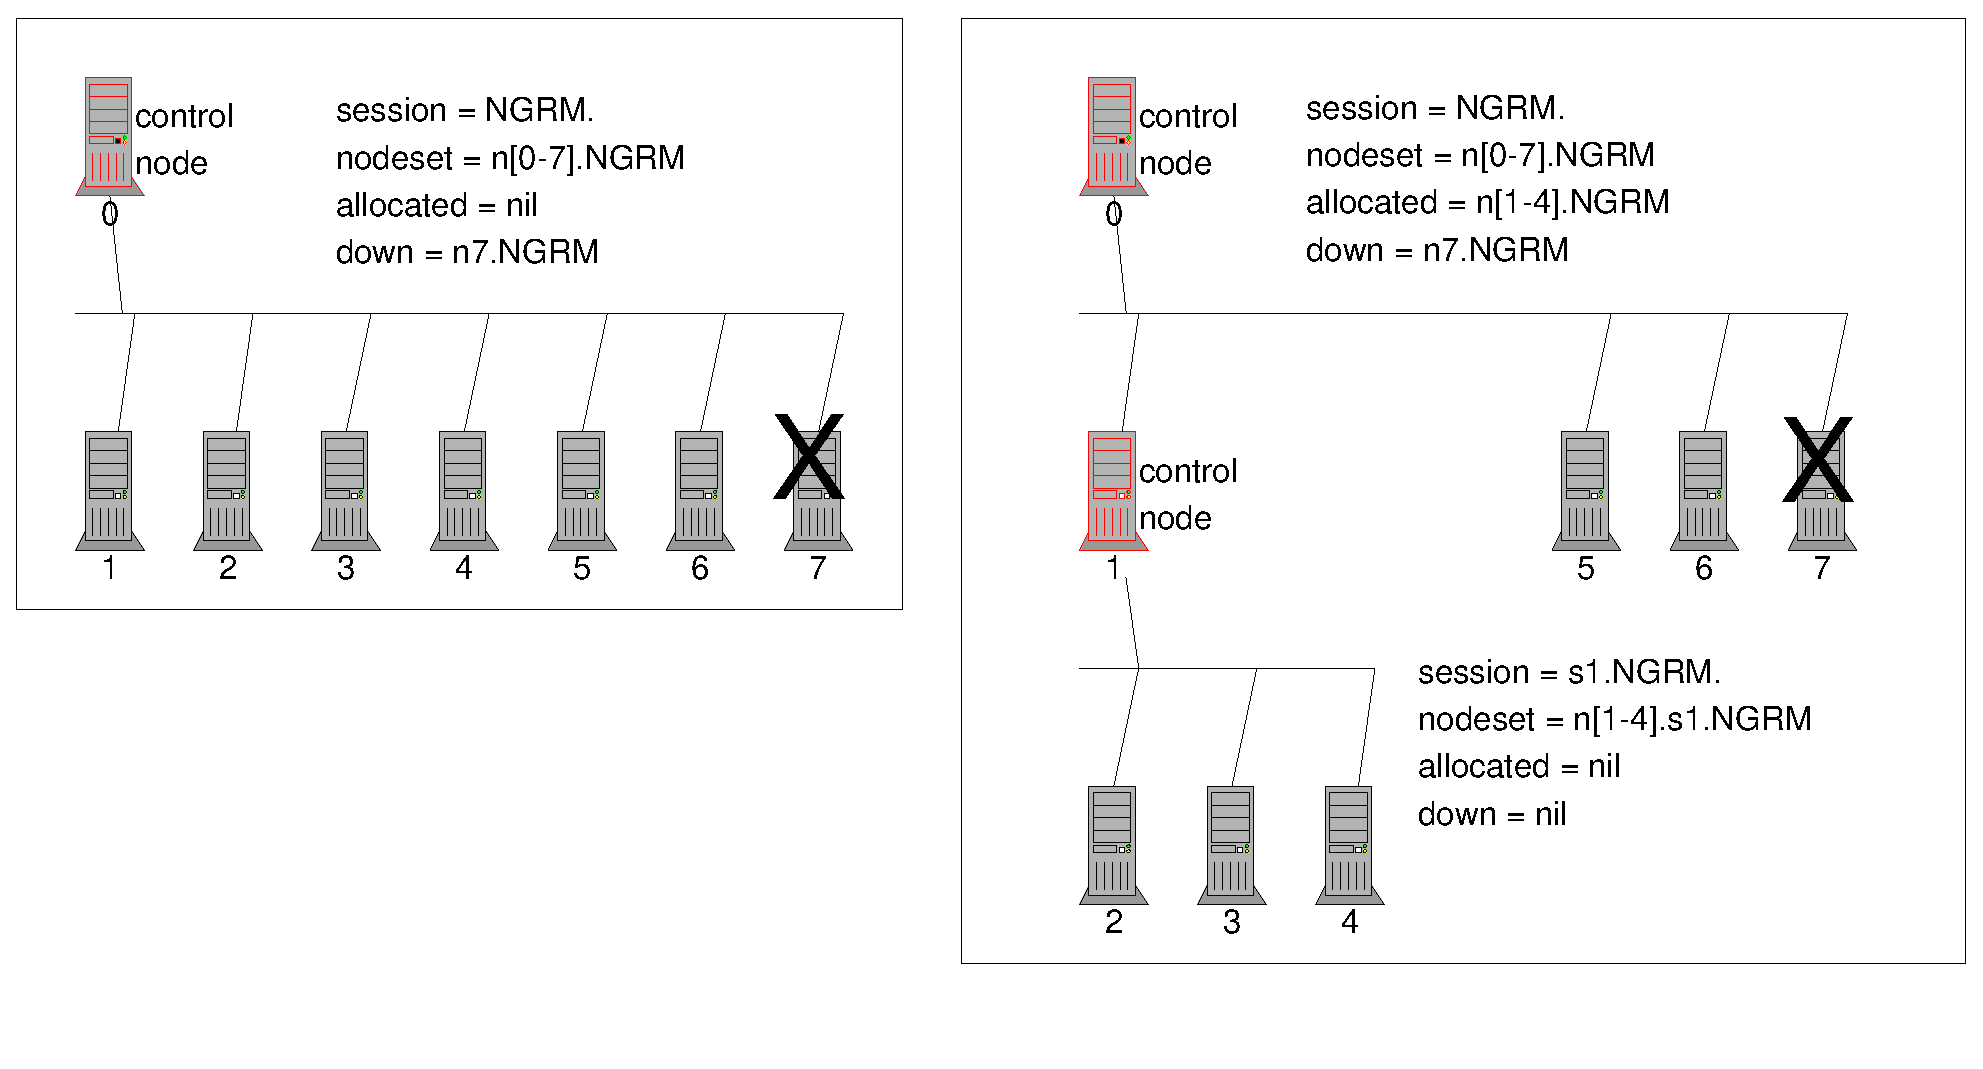
\includegraphics[scale=0.50]{cmb}
%\caption{Comms Message Broker Spawning a New Comms Session}
%\label{FigCMBSpawn}
%\end{figure}

\paragraph{Session Creation}
The CMB is responsible for the creation of
child comms sessions.
%as shown in Figure~\ref{FigCMBSpawn}.
A child session is created by building the child session state,
updating the current (parent) session state, then sending the
child control node(s) the full session state, and the rest of the nodes
just the new session key and sufficient information to wire up to their
peers in the internal toplogy.
The DNS is updated in the parent to delegate authority
for the new subdomain to the child's DNS servers.
DNS servers are bootstrapped in the child, and the resolver is updated
on member nodes to reflect the new session.

\paragraph{Session Destruction}
The CMB destroys a child comms session by sending a message to the child's
control node requesting that a shutdown event be sent out session wide.
As nodes leave the child nodeset, the parent reclaims them as described 
above in the Session Membership paragraph.
If something goes wrong, the parent can short-circuit the ``clean shutdown''
and actively reclaim nodes as above, as though they had already left the
child nodeset.
The DNS is updated in the parent to remove references to the session's
subdomain.

\subsection{Reduction Network}

\begin{figure}
\centering
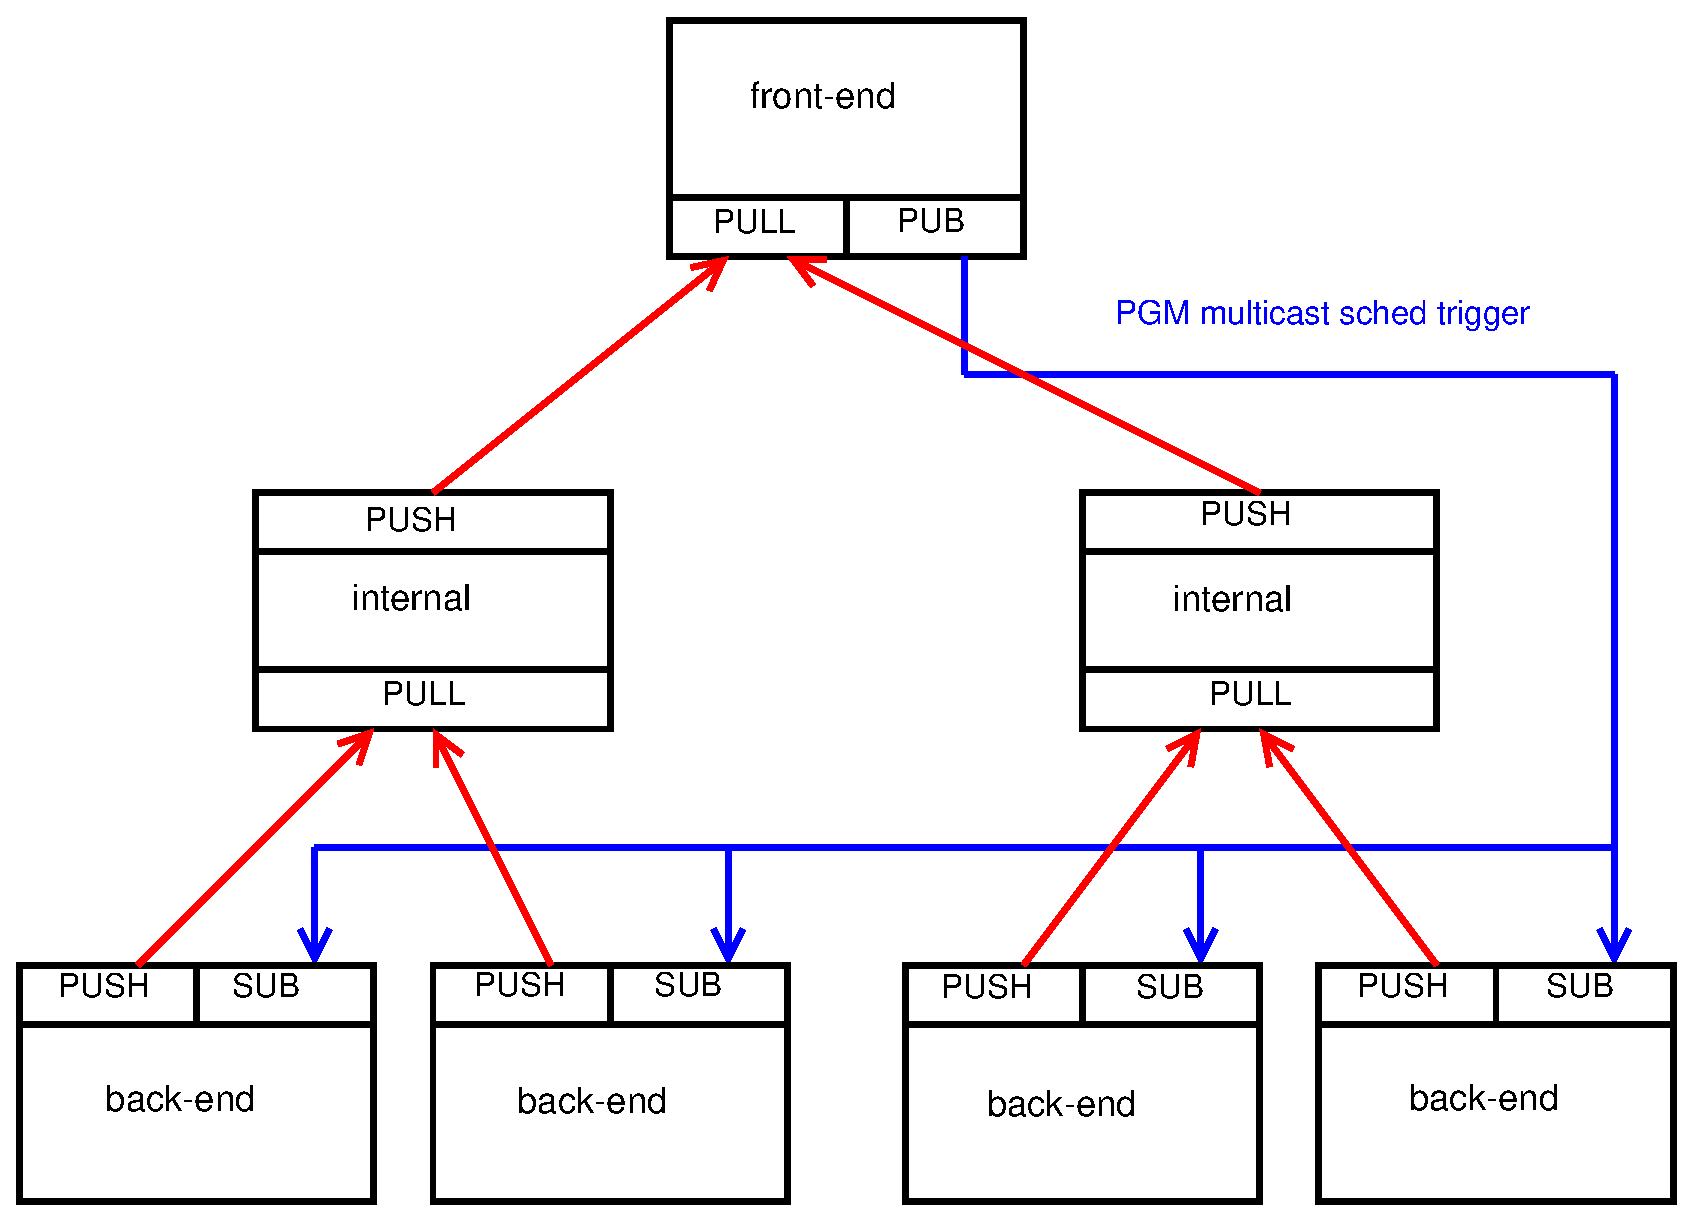
\includegraphics[scale=0.35]{comms_zmq_reduct}
\caption{Reduction network speculatively implemented with \zMQ.
A front-end node communicates with back-end nodes using PGM multicast
in the {\em downstream} direction.  {\em Upstream} traffic makes its
way from back-end nodes, through internal nodes that perform data 
reduction on messages, and on to the front-end.}
\label{FigZmqTBON}
\end{figure}

The Tree-Based Overlay Network (TB\={O}N), exemplified by MRNet~\cite{MRNet},
is regarded as a useful communications substrate for scaling
distributed debuggers and similar tools.
The \ngrm\ reduction network offers a similar capability
within a comms session for general use by distributed \ngrm\ components,
for example monitoring and stdout/stderr capture.
While MRNet is focused on portable tools that instantiate their own TB\={O}N
with a custom topology for exclusive use of the tool and tear it down when
the tool exits,
the \ngrm\ reduction network topology tracks that of the CMB,
is persistent for the life of the comms session,
and can be shared among components.
It shares the elasticity and fault-tolerance properties of the CMB.
Data passed over the reduction network ``counts'' towards CMB liveness
tracking.
The reduction network will obtain privacy and integrity using the comms
session security context.
Message handling could be accomplished with
\zMQ\ (Figure~\ref{FigZmqTBON}) or by a combination of \zMQ\ and SCTP.

\paragraph{Topology}
The reduction network topology tracks the CMB topology.
Its front-end is rooted at the control node.
Its back-ends span every node in the comms session, including those
running internal and front-end processes.
The location of internal processes will be dependent on the design of
the CMB.
Although the topology of the reduction network must have the elasticity
and fault tolerance properties of the comms session,
we anticipate that for a session in stasis, the topology will be fixed.
For example, branching factor and depth will not dynamically adjust for
performance.
However, it may be possible to set tunable parameters for the job that
would affect the initial CMB toplogy and thus that of the reduction network.

\paragraph{Downstream communiciation}
\ifcomments
\marginpar{\tiny {\bf jg:}
Is there a case for unicast store-and-forward like is used in MRNet?
Why did they choose to do it that way?  Reliable multicast (PGM) seems better
as long as the volume of data remains low.}
\fi
The reduction network utilizes IP level multicast (e.g. PGM) to send
data from the front-end to the back-ends.
As with event messages, downstream messages are a
$(tag, message)$ tuple with the tag used to distinguish different
services sharing the reduction network and to implement application-specific
addressing, for example to address a subset of back-end processes.

\paragraph{Upstream communication}
Communication from the back-ends to the front-end is the main function
of the reduction network.  It is unicast-based.  Scalability is obtained
by reductions that are performed by internal processes, for example
aggregating duplicate messages, forwarding a weighted average of discrete
samples, or simply concatenating messages.
There may be any number of levels of internal
processes, with each internal process operating on raw data or data
that has already been reduced by a previous level.
As with downstream communication, upstream messages are a
$(tag, message)$ tuple with the tag used to distinguish different
services sharing the reduction network.

\paragraph{Programming interface}
The programming interface for the reduction network is a design
activity that can be informed by the MRNet API~\cite{MRNetAPI}, however
because the reduction network is persisent and shared, it has somewhat
different requirements in that it must interface to components running
as distinct UNIX processes and be resilient to component failure.
One approach is for applications that use the reduction
network to provide a plugin that claims a message $tag$ space and implements
a {\em socket activation} scheme similar to systemd~\cite{Systemd}
or D-Bus~\cite{Dbus} that associates the tag space with named UNIX
domain sockets and/or executables at the front-end, back-end, and internal
locations.

\paragraph{Fault tolerance}
\ifcomments
\marginpar{\tiny {\bf FIXME:}
The fault tolerance strategy both for the CMB and the reduction network
is rather poorly developed in the description thus far.
At minimum it needs to be called out in the WBS as a significant R\&D activity.}
\marginpar{\tiny {\bf kim-review:}
Fault tolerance should be more fully designed in the comms
layer before moving forward.}
\fi
The CMB provides notification messages when nodes cease to respond
so that other services can manage failures.
The reduction network will use this facility and track the CMB topology
to remain functional when faults occur.
However, although we are encouraged that fault tolerance
has been achieved for certain use cases in MRNet as described by
Arnold and Miller~\cite{MrNetFail},
we recognize that it will be a challenge to design our reduction network
to be generally reliable and fault-tolerant.
Therefore we leave the possibility open that the design will provide
these attributes only for selected use cases and failure modes.

\ifwbs
\newpage
\subsection{Communication Framework WBS}\label{CommsFrameworkWBS}

\begin{longtable}{|p{1cm}|p{10.2cm}|p{1cm}|p{1cm}|p{1.8cm}|}\hline
  \textbf{Item} & \textbf{Description}
		& \textbf{Deliv}\footnote{SD = software drop,
			DR = design review, V = viewgraphs, D = document}
		& \textbf{Weeks} & \textbf{Depend} \\
  \hline
  \hline
  \multicolumn{5}{|l|}{1.1. \textbf{Comms Toolkit}} \\
  \hline
  1.1.1.  & \zMQ\ evaluation.
          Consider CMB and aggregation/reduction design based on \zMQ.
          How does PGM implement reliable message delivery?
          Is the connectionless model a serious problem? 
          Is the implementation robust?
          How would security be integrated?
	& V
	& 2
	& \\
  \hline
  1.1.2.  & SCTP evaluation.
          Consider CMB and aggregation/reduction framework design based on SCTP.
          Compare performance with \zMQ.
          Is the Linux SCTP implementation robust?
          How would security model be integrated?
	& V
	& 4
	& \\
  \hline
  1.1.3.  & MUNGE key change capability to make large MUNGE realm manageable.
	  Add support for transitioning to a new key\footnote{
	  \url{https://code.google.com/p/munge/issues/detail?id=19}}.
	& SD
	& 
	& \\
  \hline
  1.1.4.  & Design fully routed management and IB networks for all
          Linux clusters in the Livermore Computing collaboration zone.
          Evaluate DNS, DHCP, and MADCAP (or alternative) software
	  and develop deployment strategy.
          Design should be reviewed by LC networking and security staff
	  and published as model for similar efforts.
	& V
	& 
	& \\
  \hline
  1.1.5.  & Investigate IPsec scalability for a comms session.
          Can Linux IPsec implementation handle 100K security association
	  (SA) table entries?
	& V
	&
	& \\
  \hline
  \multicolumn{5}{|l|}{1.2. \textbf{Comms Message Broker}} \\
  \hline
  1.2.1.  & CMB I design/prototype.  Develop CMB API's and a protoype
          implementation with a centralized architecture that scales
          to approx 256 nodes.   Stablize API's and allow dependent
	  development to proceed.  Replace "whatsup" Cerebro tool on hype.
	& DR, SD, V
	&  
	& 1.1.1, 1.1.2, 1.1.5 \\
  \hline
  1.2.2.  & Document CMB API's and comms toolkit usage for \ngrm\ components.
          Develop toy application(s) demonstrating usage.
	& V, D
	&  
	& 1.1.1, 1.1.2, 1.1.5, 1.2.1 \\
  \hline
  1.2.3.  & CMB II design/prototype.  Design/prototype CMB II 
          implementation with a distributed architecture that scales
          to 100K nodes.   No fault tolerance.
	& DR, SD, V
	&  
	& 1.1.3, 1.1.4, 1.2.2 \\
  \hline
  1.2.4.  & CMB III design/develop.  Final implementation with full
	  scalability and fault tolerance.
	& DR, SD, V
	&  
	& 1.2.3 \\
  \hline
  \multicolumn{5}{|l|}{1.3. \textbf{Aggregation/Reduction Network Overlay}} \\
  \hline
  1.3.1.& aggregation/reduction framework design/prototype.
	& DR
	&
	& 1.2.2\\
  \hline
  1.3.2.& Implement aggregation/reduction framework.
	& SD
	&
	& 1.3.1\\
  \hline
\end{longtable}
\fi
